\sisetup{locale = EN} 
%%%%%%%%%%%%%%%%%%%%%%%%%%%%%%%%%%%%%%%%%%%%%%%%%%%%%%%%%%%%%%%%%%%%%%%%%%%%%%%%%%%%%%%%%%%%%%
%
%   ENGLISH
%
%%%%%%%%%%%%%%%%%%%%%%%%%%%%%%%%%%%%%%%%%%%%%%%%%%%%%%%%%%%%%%%%%%%%%%%%%%%%%%%%%%%%%%%%%%%%%%
\usetikzlibrary {arrows.meta}


\title{\textbf{\rmfamily Introductory Lecture}}
\subtitle{\horrorfont The Standard Model of particle physics and the LHCb detector}
\author[~\WorkGroup~]{{\WorkGroup}}
\institute[\WorkGroup]{ \University}

%%%%%%%%%%%%%%%%%%%%%%%%%%%%%%%%%%%%%%%%%%%%%%%%%%%%%%%%%%%%%%%%%%%%%%%%%%%%%%%%%%%%%%%%%%%%%%
%   Options for the footline
%%%%%%%%%%%%%%%%%%%%%%%%%%%%%%%%%%%%%%%%%%%%%%%%%%%%%%%%%%%%%%%%%%%%%%%%%%%%%%%%%%%%%%%%%%%%%%
\setbeamertemplate{footline}
{
\leavevmode%
\hbox{%
\begin{beamercolorbox}[wd=0.5\paperwidth,ht=2.25ex,dp=1ex,center]{author in foot}%
\usebeamerfont{author in foot} \parbox{0.5\paperwidth}{\insertsubsection{}}
\end{beamercolorbox}%
\begin{beamercolorbox}[wd=0.11\paperwidth,ht=2.25ex,dp=1ex,center]{title in head/foot}%
\usebeamerfont{title in head/foot}
\end{beamercolorbox}%
\begin{beamercolorbox}[wd=0.385\paperwidth,ht=2.25ex,dp=1ex,right]{date in head/foot}%
\usebeamerfont{date in head/foot}\insertsection{}\hfill
|~Slide \insertframenumber{} \hspace*{2ex}%/ \inserttotalframenumber\hspace*{2ex}
\end{beamercolorbox}}%
\vskip0pt%
}

%%%%%%%%%%%%%%%%%%%%%%%%%%%%%%%%%%%%%%%%%%%%%%%%%%%%%%%%%%%%%%%%%%%%%%%%%%%%%%%%%%%%%%%%%%%%%%
% Options for the timetable
%%%%%%%%%%%%%%%%%%%%%%%%%%%%%%%%%%%%%%%%%%%%%%%%%%%%%%%%%%%%%%%%%%%%%%%%%%%%%%%%%%%%%%%%%%%%%%

% \makeatletter
% \newcommand{\setcurrtime}[1]{%
%   \set@time\curr@hour\curr@mins#1\@nil
% }
% \def\set@time#1#2#3:#4\@nil{%
%   \def#1{#3}\def#2{#4}%
% }
% \newcommand{\currtime}[1][00:00]{%
%   \begingroup
%   \set@time\new@hour\new@mins#1\@nil
%   \count\z@=\curr@mins\relax
%   \count\tw@=\curr@hour\relax
%   \advance\count\z@\new@mins\relax
%   \advance\count\tw@\new@hour\relax
%   \ifnum\count\z@>59
%     \advance\count\z@-60
%     \advance\count\tw@\@ne
%   \fi
%   % we have to use \count\z@ and \count\tw@ before
%   % ending the group and printing the result
%   \edef\x{\endgroup\two@digits{\count\tw@}:\two@digits{\count\z@}}\x
% }
% \makeatother


%%%%%%%%%%%%%%%%%%%%%%%%%%%%%%%%%%%%%%%%%%%%%%%%%%%%%%%%%%%%%%%%%%%%%%%%%%%%%%%%%%%%%%%%%%%%%%
%%%%%%%%%%%%%%%%%%%%%%%%%%%%%%%%%%%%%%%%%%%%%%%%%%%%%%%%%%%%%%%%%%%%%%%%%%%%%%%%%%%%%%%%%%%%%%

\begin{document}\selectlanguage{english}


%%%%%%%%%%%%%%%%%%%%%%%%%%%%%%%%%%%%%%%%%%%%%%%%%%%%%%%%%%%%%%%%%%%%%%%%%%%%%%%%%%%%%%%%%%%%%%
\begin{frame}{\small \hfill \textcolor{gray}{Today you are Scientists!}}
\, \vspace{0.1cm}  \Large  \begin{center}
    \textbf{Welcome to the Masterclass!} 
\end{center} 
  \small \, \vspace{1cm} \\
    \emph{Please be patient a little longer. The event will start shortly.}
\end{frame}
%%%%%%%%%%%%%%%%%%%%%%%%%%%%%%%%%%%%%%%%%%%%%%%%%%%%%%%%%%%%%%%%%%%%%%%%%%%%%%%%%%%%%%%%%%%%%%
\section{}
%%%%%%%%%%%%%%%%%%%%%%%%%%%%%%%%%%%%%%%%%%%%%%%%%%%%%%%%%%%%%%%%%%%%%%%%%%%%%%%%%%%%%%%%%%%%%%
\begin{frame}
\begin{minipage}[t]{0.4\textwidth}
    \includegraphics[width=\textwidth]{Figures Introductory Lecture/Introduction/Human.png}
\end{minipage}
\begin{minipage}[t]{0.43\textwidth}
   \vspace{-3cm} \centering
     \Large{ \textbf{What are humans actually made of?}} \\ \vspace{0.5cm} \normalsize{And,} \\ \Large \textbf{how do we know that?} % Meldung der SuS sammeln 
\end{minipage}  
\end{frame}
%%%%%%%%%%%%%%%%%%%%%%%%%%%%%%%%%%%%%%%%%%%%%%%%%%%%%%%%%%%%%%%%%%%%%%%%%%%%%%%%%%%%%%%%%%%%%%
\begin{frame}
    \begin{center}
    \Large \textbf{What is the world made of?} \\
    \vspace{1cm}
   \textbf{Why is it built the way it is?}\\
     \vspace{1cm}
        \large Today we would like to explore the question: \\ 
    \Large  \textbf{What is matter and how can it be "measured"?}
    \end{center}
    \end{frame}

%%%%%%%%%%%%%%%%%%%%%%%%%%%%%%%%%%%%%%%%%%%%%%%%%%%%%%%%%%%%%%%%%%%%%%%%%%%%%%%%%%%%%%%%%%%%%%

\begin{frame}[plain]
\begin{center}
    \begin{tabular}{ccc}
 \parbox{0.33\textwidth}{\LogoInsitute}    &
 ~~~~\parbox{0.33\textwidth}{\includegraphics[height=1cm]{Logos And Group/LHCb_Logo.png}}   &  \parbox{0.33\textwidth}{\LogoUniversity}\\
\end{tabular}
\end{center}

\maketitle
\end{frame}
%%%%%%%%%%%%%%%%%%%%%%%%%%%%%%%%%%%%%%%%%%%%%%%%%%%%%%%%%%%%%%%%%%%%%%%%%%%%%%%%%%%%%%%%%%%%%%

\GroupPresentation \addtocounter{framenumber}{1}

%%%%%%%%%%%%%%%%%%%%%%%%%%%%%%%%%%%%%%%%%%%%%%%%%%%%%%%%%%%%%%%%%%%%%%%%%%%%%%%%%%%%%%%%%%%%%%
\begin{frame}{Who are you?}
\Large Who are we? \textcolor{green}{\ding{52}} \\ \vspace{1cm}
    \Large Who are you? \\
    \large ~ \ding{43} Attendance sheet
\end{frame}
%%%%%%%%%%%%%%%%%%%%%%%%%%%%%%%%%%%%%%%%%%%%%%%%%%%%%%%%%%%%%%%%%%%%%%%%%%%%%%%%%%%%%%%%%%%%%%
\begin{frame}{\textbf{What is Matter and how can it be "Measured"?}}
\begin{center}
    \Large What do we need to know in order to answer this question?  
\end{center}
\end{frame}
%%%%%%%%%%%%%%%%%%%%%%%%%%%%%%%%%%%%%%%%%%%%%%%%%%%%%%%%%%%%%%%%%%%%%%%%%%%%%%%%%%%%%%%%%%%%%%
\begin{frame}{Today's Day}

\footnotesize
 \texttt{Put your time schedule in here.}

\end{frame}
%%%%%%%%%%%%%%%%%%%%%%%%%%%%%%%%%%%%%%%%%%%%%%%%%%%%%%%%%%%%%%%%%%%%%%%%%%%%%%%%%%%%%%%%%%%%%%
% \begin{frame}{Motivation}
% We start with the scale picture, using practical questions to get to microscopic regime 
%     - "What is it made of and how do we know it?"   %%% Hier ist darauf zu achten, dass die Messaperaturen besprochen werden: Auge, Licht, Mikroskop ... etc. Bereitet Grundlegendes Verständig für Detektoren vor
% \end{frame}
% \begin{frame}{How do we measure matter?}
%     We motivate the students to answer the question themselves
% \end{frame}
%%%%%%%%%%%%%%%%%%%%%%%%%%%%%%%%%%%%%%%%%%%%%%%%%%%%%%%%%%%%%%%%%%%%%%%%%%%%%%%%%%%%%%%%%%%%%%
\section{Introduction into particle physics}
%%%%%%%%%%%%%%%%%%%%%%%%%%%%%%%%%%%%%%%%%%%%%%%%%%%%%%%%%%%%%%%%%%%%%%%%%%%%%%%%%%%%%%%%%%%%%%
\begin{frame}[plain]
   \begin{center} 
  \huge{  \ding{182} }\\
   \Large{Introduction to particle physics}
\end{center}
\end{frame}
%%%%%%%%%%%%%%%%%%%%%%%%%%%%%%%%%%%%%%%%%%%%%%%%%%%%%%%%%%%%%%%%%%%%%%%%%%%%%%%%%%%%%%%%%%%%%%
\begin{frame}[t]{And what is actually in the nucleus?}

    \begin{minipage}{\linewidth}
        \begin{minipage}{0.33\linewidth}
             \qquad Atom 
        \end{minipage}     
        \begin{minipage}{0.4\linewidth}
             \quad Atomic nuclei 
        \end{minipage}    
        \begin{minipage}{0.24\linewidth}
            \quad\textbf{Quarks}
        \end{minipage}    
    \end{minipage} \vspace{0.5cm}
    
     \begin{minipage}{0.99\linewidth}
        \begin{figure}
            \centering
            \includegraphics[width=\textwidth]{Figures Introductory Lecture/Standard Model/Scale_Atom_Quark_noText_2.png}
           % \caption{Caption}
            \label{fig:scale_atom_qaurk}
        \end{figure}
     \end{minipage}  
     \vspace{-15cm}
    \begin{minipage}{\linewidth}
        \begin{minipage}{0.33\linewidth}
            \qquad \Large $10^{-10}$\,m
        \end{minipage}     
        \begin{minipage}{0.33\linewidth}
             \quad \Large $10^{-15}$\,m
        \end{minipage}    
        \begin{minipage}{0.29\linewidth}
            \quad \Large $\leq10^{-18}$\,m
        \end{minipage}    
    \end{minipage}

\end{frame}
%%%%%%%%%%%%%%%%%%%%%%%%%%%%%%%%%%%%%%%%%%%%%%%%%%%%%%%%%%%%%%%%%%%%%%%%%%%%%%%%%%%%%%%%%%%%%%
%\begin{frame}{Quark im Nukleus?!}
%    Picture von dem Milchprodukt in verschiedenen Geschmäckern
%\end{frame}
%%%%%%%%%%%%%%%%%%%%%%%%%%%%%%%%%%%%%%%%%%%%%%%%%%%%%%%%%%%%%%%%%%%%%%%%%%%%%%%%%%%%%%%%%%%%%%
%\begin{frame}<presentation:0>{Theorie/Quarks - Hannah}
%    Here should be the typical scale picture. We start with an atom and move to quarks via nuclei and protons/neutrons. (Magnefying glass on proton/neutron and show the quarks) 
    
%    Goal: Students know that the proton consists of three subparticles. Two of these are identical (AAB (uud) and BBA (ddu)) 
%\end{frame}


%\begin{frame}<presentation:0>{Weiteres - Hannah}
%    Eventuell vergleich von theoretischer und experimentalphysik ziehen und für das Forschungsgebiet um die Starke Wechselwirkung ableiteten, dass beide Hand in Hand gehen müssen ("Blackbox").
%\end{frame}
%%%%%%%%%%%%%%%%%%%%%%%%%%%%%%%%%%%%%%%%%%%%%%%%%%%%%%%%%%%%%%%%%%%%%%%%%%%%%%%%%%%%%%%%%%%%%%

\begin{frame}{Quarks - What's that?}

    \begin{minipage}[t]{\linewidth}\raggedleft
          What charge has a \textcolor{red}{\textbf{neutron}}/\textcolor{blue}{\textbf{proton}}? \\
           What charge have \textcolor{darkgreen}{\textbf{Q}}\textbf{u}\textcolor{darkgreen}{\textbf{a}}\textbf{r}\textcolor{darkgreen}{\textbf{k}}\textbf{s}?
    \end{minipage}%
    \vspace{-0.6cm}
    \begin{minipage}{\linewidth}\raggedright
        \begin{figure}[htb]
            \includegraphics[width=0.79\textwidth]{Figures Introductory Lecture/Standard Model/Quarks.png}
            %\caption{}
            \label{fig:quarks}
        \end{figure}            
    \end{minipage}
    
\end{frame}
%%%%%%%%%%%%%%%%%%%%%%%%%%%%%%%%%%%%%%%%%%%%%%%%%%%%%%%%%%%%%%%%%%%%%%%%%%%%%%%%%%%%%%%%%%%%%%

%\begin{frame}{Quarks - Was ist das?}
%Here we introduce the quarks. We know the proton/neutron has 3 subparticles. Students should know the electric charge of proton/neutron. How can we combine 3 particles to form an electric positive and neutral particle. 

%Goal: quark composition of proton/neutron. No need to mention up and down yet
%\end{frame}
%%%%%%%%%%%%%%%%%%%%%%%%%%%%%%%%%%%%%%%%%%%%%%%%%%%%%%%%%%%%%%%%%%%%%%%%%%%%%%%%%%%%%%%%%%%%%%
\begin{frame}{How do Quarks Stick Together?}  
    \begin{figure}[htb]
        \includegraphics[width=1\textwidth]{Figures Introductory Lecture/Standard Model/StrongForce_EM.png}
        %\caption{}
        \label{fig:strong_force_1}
    \end{figure} \\
    \Large \begin{center}
        The electromagnetic force \emph{could} bind quarks!
    \end{center}
\end{frame}
%%%%%%%%%%%%%%%%%%%%%%%%%%%%%%%%%%%%%%%%%%%%%%%%%%%%%%%%%%%%%%%%%%%%%%%%%%%%%%%%%%%%%%%%%%%%%%
% Zweiter Satz als Gegenfrage .. Aber warum halten Protonen zusammen? 
\begin{frame}{Forces in Atomic Nuclei}
...but why do \emph{atomic nuclei} hold together?!\\ \, \hspace{2cm} \ding{43} \textcolor{blue}{\textbf{Protons}} repel each other electromagnetically!

    \begin{figure}[htb]
        \includegraphics[width=0.3\textwidth]{Figures Introductory Lecture/Standard Model/Nukleus.png}
        %\caption{}
        \label{fig:strong_force_2}
    \end{figure}\\
    \ding{43} There is another force that binds atomic nuclei\\ 
    \vspace{0.5cm}\begin{center}
    \Large{The \textbf{strong force}}
    \end{center}
\end{frame}
%%%%%%%%%%%%%%%%%%%%%%%%%%%%%%%%%%%%%%%%%%%%%%%%%%%%%%%%%%%%%%%%%%%%%%%%%%%%%%%%%%%%%%%%%%%%%%
% Protonen -> B
\begin{frame}{Proton Question Time}
\begin{center} \Large
        ...but, \\ how can we determine whether protons are held together by the\\ strong or electromagnetic force\\? 
\end{center}

\end{frame}
%%%%%%%%%%%%%%%%%%%%%%%%%%%%%%%%%%%%%%%%%%%%%%%%%%%%%%%%%%%%%%%%%%%%%%%%%%%%%%%%%%%%%%%%%%%%%%
% Graue Kreise dunkler machen -> keine chance auf dem Beamer
% Masse weg
% u und d an quarks dranschreiben, oder im Text einbauen
\begin{frame}{Other Quark Combinations}
In fact, we find particles that consist of three up quarks/three down quarks!
    \begin{figure}[htb]
        \includegraphics[width=0.6\textwidth]{Figures Introductory Lecture/Standard Model/DeltaBaryons.png}
        %\caption{}
        \label{fig:strong_force_2}
    \end{figure}
    $\hspace{3cm}\rightarrow \Delta^{++}$\hspace{3cm} $\rightarrow \Delta^{-}$\\ \vspace{0.5cm}
    \ding{43} The \textbf{strong force} must be responsible for the binding!
    % only speakting about strong force, not SM here.
\end{frame}
%%%%%%%%%%%%%%%%%%%%%%%%%%%%%%%%%%%%%%%%%%%%%%%%%%%%%%%%%%%%%%%%%%%%%%%%%%%%%%%%%%%%%%%%%%%%%%
\begin{frame}{Differences of the Forces}
What is the difference between the electromagnetic force and the strong force?
\pause
\begin{itemize}
    % Die EM Kraft ist spürbar!
    \item We don't feel the strong force in everyday life
    \item The strong force attracts electrically neutral \& charged particles
    \item ...
    \item[\ding{43}] We understand the electromagnetic force, but we have a harder time with the strong force!
    % Fragen ob den Leuten noch was einfällt...
\end{itemize}
\end{frame}
%%%%%%%%%%%%%%%%%%%%%%%%%%%%%%%%%%%%%%%%%%%%%%%%%%%%%%%%%%%%%%%%%%%%%%%%%%%%%%%%%%%%%%%%%%%%%%
% die auf sie wirkt...
% Quarks müssen eine weitere Ladung haben -> Farbladung
% Wir messen die Farbladung nicht
\begin{frame}{The Properties of the Strong Interaction} 
For the \textbf{strong force} there is a \textbf{charge} on which it acts! \\
\begin{itemize}
\begin{itemize}
    \item [\ding{220}] Quarks must have a so-called \textbf{colour charge}\\\
    \item[] But the particles we observe are colourless! \\
    \end{itemize}
   \item[] \textbf{Visualisation:}
\end{itemize} \vspace{-0.5cm}
    \begin{figure}[htb]                                                 
    \includegraphics[width=0.8\textwidth]{Figures Introductory Lecture/Standard Model/GrayAdditiveColours.png}          
    %\caption{}                                                         
    \label{fig:strong_force_3}                                         
    \end{figure} \vspace{-0.5cm}
    \ding{220} Overall colour-neutral particles!
\end{frame} 
%%%%%%%%%%%%%%%%%%%%%%%%%%%%%%%%%%%%%%%%%%%%%%%%%%%%%%%%%%%%%%%%%%%%%%%%%%%%%%%%%%%%%%%%%%%%%%
\begin{frame}{The Standard Model of Particle Physics}
% Idea is to show first only the particles student should know from the last slides, i.e. u and d quark. Then ask, what other elementary particles they might know of (expect electron and photon).
% From there talk about how physicists made the "strange" discovery of new particles that did not seem to be compsed out of ud only -> discovered more flavours over past decays, explain the three generations with increasing mass, same for leptons.
%In the end ask but how is it possible that the matter surrounding us is only made up of p,n ie ud quarks? -> Heavier flavoured particles must decay into first generation
\foreach \n in {1,...,4}{
    \includegraphics<\n>[width=0.9\textwidth]{Figures Introductory Lecture/Standard Model/ENG_SM_\n.png}%
}
%%%%%%%%%%%%%%%%%%%%%%%%%%%%%%%%%%%%%%%%%%%%%%%%%%%%%%%%%%%%%%%%%%%%%%%%%%%%%%%%%%%%%%%%%%%%%%
\end{frame}
\begin{frame}{The Standard Model of Particle Physics}
    \includegraphics[width=0.9\textwidth]{Figures Introductory Lecture/Standard Model/ENG_SM2_1.png}
\end{frame}
%%%%%%%%%%%%%%%%%%%%%%%%%%%%%%%%%%%%%%%%%%%%%%%%%%%%%%%%%%%%%%%%%%%%%%%%%%%%%%%%%%%%%%%%%%%%%%

% \begin{frame}{Die schwache Wechselwirkung}
% % So how can we imagine such a decay? Lefthand side shows such a "strange" particle, what do we have to change to go a proton, is there something missing (charge) so need electrn for the decay.
% % More physical picture: show feynman diagram introduce bosons as mediators of interaction.
% \only<1>{
% \begin{figure}[htb]
%     \includegraphics[width=0.9\textwidth]{Figures Introductory Lecture/Standard Model/LambdaDecay.png}%
%     %\caption{}
%     \label{fig:LambdaToProton}
% \end{figure}
% }
% \only<2>{
% \begin{figure}[htb]
%     \includegraphics[width=0.9\textwidth]{Figures Introductory Lecture/Standard Model/LambdaDecayCharge.png}%
%     %\caption{}
%     \label{fig:Lambda_Decay}
% \end{figure}
% }
% \only<3>{
% \begin{figure}[htb]
%     \includegraphics[width=0.9\textwidth]{Figures Introductory Lecture/Standard Model/LambdaDecayFull.png}%
%     %\caption{}
%     \label{fig:Lambda_DecayFull}
% \end{figure}
% }
% \end{frame}




\begin{frame}{The Week Force}
\begin{center}
    

    \begin{tikzpicture}[scale=0.9]
 
          \fill[orange] (0,0) circle (2) node [left=60pt,white] {\LARGE $\Lambda^0$};
          \fill[upQuark] (-0.75,-0.75) circle (0.5)  node[black] {\Large $u$};
            \fill[downQuark] (0.75,-0.75) circle (0.5)  node[white] {\Large$d$};
            \fill[strangeQuark] (0,0.75) circle (0.5)  node[black] {\Large$s$};

             \fill[Proton] (7,1) circle (2) node [right=60pt, white] {\LARGE $p$} ;
        \fill[upQuark] (6.25,0.25)circle (0.5)  node[black] {\Large$u$};
             \fill[upQuark] (7,1.75)circle (0.5)  node[black] {\Large$u$};
              \fill[downQuark] (7.75,0.25)circle (0.5)  node[white] {\Large$d$} ;


       % \fill[Elektron] (7.1,-2) circle (0.3) node[black] {$e^-$};


       % \fill[black] (6,-3) circle (0.05) node[right] {$\Bar{\nu}_e$};

        \draw[-{Latex[length=5mm]}, line width=1mm] (2.1,0.1) to (4.9,0.9){};
        %\draw[-{Latex[length=5mm]}, line width=1mm] (2.1,0) to (6.5,-1.8){};
      %  \draw[-{Latex[length=5mm]}, line width=1mm] (2.1,-0.1) to (5.9,-2.9){};
              
            
%Controling Points
\fill[white] (-3,-4) circle (0.1);
\fill[white] (10,3) circle (0.1);
    \end{tikzpicture}
    \end{center}
\end{frame}




\begin{frame}{The Week Force}\addtocounter{framenumber}{-1}
\begin{center}
    

    \begin{tikzpicture}[scale=0.9]
 
        \fill[orange] (0,0) circle (2) node [left=60pt,black] {\LARGE $\Lambda^0$};
            \fill[upQuark] (-0.75,-0.75) circle (0.5)  node[black] {\Large $u$};
            \fill[downQuark] (0.75,-0.75) circle (0.5)  node[white] {\Large$d$};
            \fill[strangeQuark] (0,0.75) circle (0.5)  node[black] {\Large$s$};

        \fill[Proton] (7,1) circle (2) node [right=60pt, black] {\LARGE $p$} ;
            \fill[upQuark] (6.25,0.25)circle (0.5)  node[black] {\Large$u$};
             \fill[upQuark] (7,1.75)circle (0.5)  node[black] {\Large$u$};
              \fill[downQuark] (7.75,0.25)circle (0.5)  node[white] {\Large$d$} ;


        %\fill[Elektron] (7.1,-2) circle (0.3) node[black] {$e^-$};


        %\fill[black] (6,-3) circle (0.05) node[right] {$\Bar{\nu}_e$};

        \draw[-{Latex[length=5mm]}, line width=1mm] (2.1,0.1) to (4.9,0.9){};
      %  \draw[-{Latex[length=5mm]}, line width=1mm] (2.1,0) to (6.5,-1.8){};
        %\draw[-{Latex[length=5mm]}, line width=1mm] (2.1,-0.1) to (5.9,-2.9){};
              
            
%Controling Points
\fill[white] (-3,-4) circle (0.1);
\fill[white] (10,3) circle (0.1);
    \end{tikzpicture}
    \end{center}
\end{frame}

\begin{frame}{The Week Force}\addtocounter{framenumber}{-1}
\begin{center}
    

    \begin{tikzpicture}[scale=0.9]
 
        \fill[orange] (0,0) circle (2) node [left=60pt,black] {\LARGE $\Lambda^0$};
            \fill[upQuark] (-0.75,-0.75) circle (0.5)  node[black] {\Large $u$};
            \fill[downQuark] (0.75,-0.75) circle (0.5)  node[white] {\Large$d$};
            \fill[strangeQuark] (0,0.75) circle (0.5)  node[black] {\Large$s$};

        \fill[Proton] (7,1) circle (2) node [right=60pt, black] {\LARGE $p$} ;
            \fill[upQuark] (6.25,0.25)circle (0.5)  node[black] {\Large$u$};
             \fill[upQuark] (7,1.75)circle (0.5)  node[black] {\Large$u$};
              \fill[downQuark] (7.75,0.25)circle (0.5)  node[white] {\Large$d$} ;


        \fill[Elektron] (7.1,-2) circle (0.3) node[black] {$e^-$};


        \fill[black] (6,-3) circle (0.05) node[right] {$\Bar{\nu}_e$};

        \draw[-{Latex[length=5mm]}, line width=1mm] (2.1,0.1) to (4.9,0.9){};
        \draw[-{Latex[length=5mm]}, line width=1mm] (2.1,0) to (6.5,-1.8){};
        \draw[-{Latex[length=5mm]}, line width=1mm] (2.1,-0.1) to (5.9,-2.9){};
              
            
%Controling Points
\fill[white] (-3,-4) circle (0.1);
\fill[white] (10,3) circle (0.1);
    \end{tikzpicture}
    \end{center}
\end{frame}

%%%%%%%%%%%%%%%%%%%%%%%%%%%%%%%%%%%%%%%%%%%%%%%%%%%%%%%%%%%%%%%%%%%%%%%%%%%%%%%%%%%%%%%%%%%%%%
\begin{frame}{Feynman Diagrams}
% Anstelle solcher Kugel Pictureer verwenden Physiker:innen Feynman diagramme
\begin{center}
\begin{tikzpicture}
\begin{feynman}
    \vertex(ul) {\(u\)};
    \vertex[right=5cm of ul] (ur) {\(u\)};
    \vertex[below=0.75cm of ul] (dl) {\(d\)};
    \vertex[right=5cm of dl] (dr) {\(d\)};
    \vertex[below=0.75cm of dl] (sl) {\(s\)};
    \vertex[right=5cm of sl] (ur2) {\(u\)};
    \vertex[right=2cm of sl] (W1);
    \vertex[below right = 1cm and 1.5cm of W1] (W2);
    \vertex[below = 0.5cm of ur2] (e) {\(e^-\)};
    \vertex[below = 1cm of e] (nue) {\(\bar \nu_e\)};
    \diagram* { {[edges=fermion]
    (ul) -- (ur), (dl) -- (dr), (sl) -- (ur2),
    (W2) -- (e), (nue) -- (W2)};
    (W1) -- [boson, edge label' = \(W^-\)] (W2)
    };
\draw [decoration={brace}, decorate]  (sl.south west) -- (ul.north west) node [pos=0.5, left] {\(\Lambda^0\)};
\draw [decoration={brace}, decorate] (ur.north east) --  (ur2.south east) node [pos=0.5, right] {\(p^+\)};
\end{feynman}
\end{tikzpicture}   
\end{center}
\ding{43} Only the weak interaction is able to change the \textbf{flavour} of a particle! 
\end{frame}
%%%%%%%%%%%%%%%%%%%%%%%%%%%%%%%%%%%%%%%%%%%%%%%%%%%%%%%%%%%%%%%%%%%%%%%%%%%%%%%%%%%%%%%%%%%%%%%


\begin{frame}[fragile]{The Standard Model of Particle Physics II}
% Show the full SM, talk about bosons as mediators, maybe the example of two people on skateboards throwing a ball, as example for repulsive force via mediating particle?

    % - Higgs und Fragen zur Gravitation vorbereiten? -> würde ich weglassen, nicht wirklich relevant, eher das Higgs kurz erwähnen als das elementarteilchen das als letztes gefunden wurde und den Punkt machen, dass Teilchenphysik aktuell ist und nicht nur experimente von vor 100 Jahren

\foreach \n in {1,...,9}{
        \includegraphics<\n>[width=0.9\textwidth]{Figures Introductory Lecture/Standard Model/ENG_SM2_\n.png}%
} 
%%%%%%%%%%%%%%%%%%%%%%%%%%%%%%%%%%%%%%%%%%%%%%%%%%%%%%%%%%%%%%%%%%%%%%%%%%%%%%%%%%%%%%%%%%%%%%
\end{frame}
\begin{frame}{Standard Model: The most Important for Today}
\begin{itemize}
    \item 6 quark flavours $u$, $d$, $s$, $c$, $b$, $t$
    \item strong, weak and electromagnetic force
    \item flavour change only via weak decay
    \item exchange particle $\gamma$, $Z^0$ \& $W^{\pm}$, $g$
    \item colour charge as charge of the strong force
    \item quarks colour-charged, particles colour-neutral
    \item []
    \item[\ding{43}] Strong force not well understood and object of current research!
\end{itemize}
    
\end{frame}
%%%%%%%%%%%%%%%%%%%%%%%%%%%%%%%%%%%%%%%%%%%%%%%%%%%%%%%%%%%%%%%%%%%%%%%%%%%%%%%%%%%%%%%%%%%%%%
  \begin{frame}{What is Mmatter and how can it be "Measured"?}\Large
 And Now?
 \begin{itemize}
     \item How can we produce particles?
     \item How can we prove all this?
 \end{itemize}
\begin{center} \pause
 
But first \\ \textbf{\textcolor{red}{5\,min break :)}
}
\end{center}  
\end{frame}
%%%%%%%%%%%%%%%%%%%%%%%%%%%%%%%%%%%%%%%%%%%%%%%%%%%%%%%%%%%%%%%%%%%%%%%%%%%%%%%%%%%%%%%%%%%%%% 
   \section{LHCb detector at CERN}
\begin{frame}[plain]

\begin{center} 
  \huge{  \ding{183} }\\
   \Large{ Introduction to the LHCb detector at CERN}

\end{center}
\end{frame}
%%%%%%%%%%%%%%%%%%%%%%%%%%%%%%%%%%%%%%%%%%%%%%%%%%%%%%%%%%%%%%%%%%%%%%%%%%%%%%%%%%%%%%%%%%%%%%


\begin{frame}{A Particle Please}

    \begin{center}
   \Large We want to produce particles!\\
    
    \Large We need a lot of \textbf{\textcolor{red}{energy}} for this!
   \mathrm{ \begin{align*}
        \textcolor{red}{E} = m\cdot c^\textsf{2} 
    \end{align*}
    }
        
    \end{center}
    
\end{frame}
%%%%%%%%%%%%%%%%%%%%%%%%%%%%%%%%%%%%%%%%%%%%%%%%%%%%%%%%%%%%%%%%%%%%%%%%%%%%%%%%%%%%%%%%%%%%%%
\subsection{Picture: CERN, edited}
\begin{frame}{Welcome to CERN \& LHC}

  \begin{center}
   \Large How can the required energy be provided?
    \end{center}
    
    \begin{figure}[h]
        \centering
        \includegraphics[width=0.7\textwidth]{Figures Introductory Lecture/LHCb Detector/LHC.jpg}
        %\c%aption{https://visit.cern/node/616}
        \label{fig:CERN_LHC}
    \end{figure}
\end{frame}

%%%%%%%%%%%%%%%%%%%%%%%%%%%%%%%%%%%%%%%%%%%%%%%%%%%%%%%%%%%%%%%%%%%%%%%%%%%%%%%%%%%%%%%%%%%%%%
\begin{frame}
\begin{figure}
\begin{overpic}[width=\textwidth]{Figures Introductory Lecture/LHCb Detector/LHC.jpg}
     \put (55,43.5) {\tiny \textcolor{white}{\centering \rotatebox[]{270}{$\rightarrow$}  Geneva}}
     \put (10,39) {\tiny \textcolor{white}{Lake Geneva}}
     \put (0,50)  {\tiny \textcolor{white}{$\leftarrow$ Lausanne}}
        \put (92,5)  {\tiny \textcolor{white}{ Lyon \rotatebox[]{340}{$\rightarrow$}}}
        \put (47,54) {\tiny \textcolor{ black}{\rotatebox[]{135}{\ding{43}} Mont Blanc}}
\end{overpic}
\end{figure}
\end{frame}
%%%%%%%%%%%%%%%%%%%%%%%%%%%%%%%%%%%%%%%%%%%%%%%%%%%%%%%%%%%%%%%%%%%%%%%%%%%%%%%%%%%%%%%%%%%%%%
\begin{frame}\addtocounter{framenumber}{-1}
\begin{figure}
\begin{overpic}[width=\textwidth]{Figures Introductory Lecture/LHCb Detector/LHC+GVA.jpg}
        \put (44,43.5) {\tiny \parbox{2.5cm}{\textcolor{white}{\centering \rotatebox[]{45}{\ding{40}}  Geneva Airport\\ Runway length: 4\,km}}}
        %\put (90,36)  {\tiny \textcolor{green}{TGV}}
        \put (0,50)  {\tiny \textcolor{white}{$\leftarrow$ Lausanne}}
        \put (92,5)  {\tiny \textcolor{white}{ Lyon \rotatebox[]{340}{$\rightarrow$}}}
        \put (10,39) {\tiny \textcolor{white}{Lake Geneva}}
        \put (47,54) {\tiny \textcolor{ black}{\rotatebox[]{135}{\ding{43}} Mont Blanc}}
\end{overpic}
\end{figure}
\end{frame}
%%%%%%%%%%%%%%%%%%%%%%%%%%%%%%%%%%%%%%%%%%%%%%%%%%%%%%%%%%%%%%%%%%%%%%%%%%%%%%%%%%%%%%%%%%%%%%
\begin{frame}\addtocounter{framenumber}{-1}
\begin{figure}
\begin{overpic}[width=\textwidth]{Figures Introductory Lecture/LHCb Detector/LHC+GVA+TGV.jpg}
        \put (44,43.5) {\tiny \parbox{2.5cm}{\textcolor{white}{\centering \rotatebox[]{45}{\ding{40}} Geneva Airport\\ Runway length: 4\,km}}}
        \put (90,36)  {\tiny \textcolor{green}{TGV}}
        \put (0,50)  {\tiny \textcolor{white}{$\leftarrow$ Lausanne}}
        \put (92,5)  {\tiny \textcolor{white}{ Lyon \rotatebox[]{340}{$\rightarrow$}}}
        \put (10,39) {\tiny \textcolor{white}{Lake Geneva}}
        \put (47,54) {\tiny \textcolor{ black}{\rotatebox[]{135}{\ding{43}} Mont Blanc}}
\end{overpic}
\end{figure}
\end{frame}
%%%%%%%%%%%%%%%%%%%%%%%%%%%%%%%%%%%%%%%%%%%%%%%%%%%%%%%%%%%%%%%%%%%%%%%%%%%%%%%%%%%%%%%%%%%%%%
%\begin{frame}{Motivation of Colider experiments (Production)}
%    E=m
    %    Wir benoetigen ein Experiment um schwere Teilchen (die nicht nur u und d enthalten) zu produzieren. Hierzu brauche wir viel Energie. % Eventuell Referenz zur kleinsten Wirkung (s.o.)?
%\end{frame}

%\begin{frame}{CERN, LHC, LHCb...}
%-> how can we produce the high amount of energy we need?
%    - From E=m. Huge Energy has to go somewhere when two particles (pp) are colliding.
%    - start with linear collider than round. Synchrotron Principe
%    - charged particles in a magn. field got accelerated
%    - Proton has more energy than a.i. Electrons. (ref to Bonn: e+ e-)
    % Das intuitive Verständnis, dass bei anihilation von Elektron und Positron "Energie frei wird", kann eventuell aufRückfragen stoßen, wenn wir pp Kollision haben, insbesondere wenn wir keine See-Quarks einfürhen. Rückfragen müsste man mit einem neuen konzept entgegnen, das kann schnell in eine verwirrende richung fühen. Daher eventuell "falsche" Erklärung hier nutzen?
%\end{frame}
%%%%%%%%%%%%%%%%%%%%%%%%%%%%%%%%%%%%%%%%%%%%%%%%%%%%%%%%%%%%%%%%%%%%%%%%%%%%%%%%%%%%%%%%%%%%%%
\subsection{}
\begin{frame}{The Collision of Particles}%{Collision and Detection}
 %- Lot Energy has to go somewhere. (E=const.)
 %- Lot Energy, lot stuff, has to go somewhere. To what? Has to be figured out. -> 
The high-energy particles collide\\
\ding{43}  What happens to the energy? % Energieerhaltung
 \\ 
%event display?
% Picture ist von hier: https://www.physicsmasterclasses.org/exercises/bonn1/de/teilchenkollision.htm
% koennte noch schoener gemacht werden. Aber die Idee ist vielleicht nicht schlecht.
\begin{figure}[h]
        %\centering
       
       \includegraphics[width=0.43\textwidth]{Figures Introductory Lecture/LHCb Detector/Kollision.png}
        \label{fig:Kollision}
    \end{figure}
\end{frame}
%%%%%%%%%%%%%%%%%%%%%%%%%%%%%%%%%%%%%%%%%%%%%%%%%%%%%%%%%%%%%%%%%%%%%%%%%%%%%%%%%%%%%%%%%%%%%%
\begin{frame}{Detectives for Particles}%{LHCb}
%- Da ist was Produziert wurden, wie kann man das Nachvollziehen. 
%    - Teilcehn treffen auf Material, diese Interaktion mit Material (-Schichten) kann man nachweisen und Spuren rekonstruieren
How can we find out what happened in the collision?\\
\ \\
    \begin{figure}[h]
        %\centering

        \begin{overpic}[width=0.8\textwidth]{Figures Introductory Lecture/LHCb Detector/Detectorsignal.png}
        \put(64.5,8){\tiny \parbox{1.7cm}{\centering Readout \\ system}}
        \put(45,50){\scriptsize Detector}
        \put(44,0){\scriptsize \parbox{2.5cm}{Electrical signal}}
        
        \end{overpic}
   
    \end{figure}
% Picture kann vermutlich auch noch in schoen erstellt werden :-D
% Ich finde das Picture wunderschön

    \begin{itemize}
        \item<2-> Which signal belongs to which particle?
    \end{itemize}
    
\end{frame}
%%%%%%%%%%%%%%%%%%%%%%%%%%%%%%%%%%%%%%%%%%%%%%%%%%%%%%%%%%%%%%%%%%%%%%%%%%%%%%%%%%%%%%%%%%%%%%
%\begin{frame}{Welches Signal gehört zu welchem Teilchen?}
       %Wie kann man Teilchen anhand von Spuren unterscheiden? 
       %-> (Reminder) Ladung, Masse, Art der WW, Energie
       %-> Detektor hat verschiedene Teilce mit verschiedenen Aufgaben

%Fragende Enntwicklung: Wie kann man verschiedene Eigenschaften der Teichen herausfinden?
%\end{frame}
%%%%%%%%%%%%%%%%%%%%%%%%%%%%%%%%%%%%%%%%%%%%%%%%%%%%%%%%%%%%%%%%%%%%%%%%%%%%%%%%%%%%%%%%%%%%%%
\begin{frame}{Which Signal Belongs to which Particle?}
    

\ \\
Remember the properties of the particles you know \\
\begin{itemize}
    \item<2-> mass \hfill $m$ \hspace{6cm}\,
    \item<2-> electric charge \hfill $q$ \hspace{6cm}\,
    \item<2-> energy \hfill $E$ \hspace{6cm}\,
    \item<2-> momentum \hfill $\vec{p} $ \hspace{6cm}\,
    \item<2-> velocity \hfill $\vec{v}$ \hspace{6cm}\,
 
\ \\
    \item<3->[\ding{220}] How can we measure these properties with the LHCb detector?

    
\end{itemize}
\end{frame}
%%%%%%%%%%%%%%%%%%%%%%%%%%%%%%%%%%%%%%%%%%%%%%%%%%%%%%%%%%%%%%%%%%%%%%%%%%%%%%%%%%%%%%%%%%%%%%
% Im Folgenden ist die Überlegung: Der LHCb Detekor baut sich langsam auf. Auf den Slides sind immer die Geräte eingezeichnet und werden laufend ergänzt (Grafiken kann Lukas machen!), Außerdem hier Pictureer von den jeweligen Geräten, s. Slides von Sebastian/Klaas. Ziel ist die AbPictureung auf der Rechenaufgabe 

%idee hierfür: beispiel teilchen durch detektor folgen (z.B. b meson wegen namensgebung):
%- zerfall im velo: gute ortsauflösung
%- rich 1: impulsmessung
%- tt: verbindung zu velo spur
%- magnet: ablenken geladener teilchen
%- tracking stations: ort nach ablenkung im magnet 
%- rich2: impuls messung von höherem impuls mit anderem gas
%- ecal/ hcal: teilchen stoppen und energie messen
%- muonkammern: misst spuren von teilchen die nicht im calo gestoppt werden (kann man auch weglassen)

%idee der folgenden slides: lhcb detektor baut sich stück für stück vom kollisionspunkt an auf, jede slide hat unten die schematik vom bisherigen detektor und oben ein foto vom subdetektor, den die slide erklärt. zusätzlich hat jede slide ein paar stichpunkte zur funktionsweise des detektors. für einige slides bieten sich fragen an die schüler an (als kommentare an den stichpunkten hinterlegt) 
%%%%%%%%%%%%%%%%%%%%%%%%%%%%%%%%%%%%%%%%%%%%%%%%%%%%%%%%%%%%%%%%%%%%%%%%%%%%%%%%%%%%%%%%%%%%%%
\subsection{Picture: CERN}
\begin{frame}{Vertex Locator (VELO)}
    \begin{minipage}{0.58\textwidth}
        \begin{itemize}
        \item Positioned around the collision point
        \item Important for track reconstruction
    \end{itemize}
    \end{minipage}\hfill
    \begin{minipage}{0.38\textwidth}
        \begin{figure}[h]
        \centering
        \includegraphics[height=3 cm]{Figures Introductory Lecture/LHCb Detector/LHCb_VELO.jpg}%source: http://cds.cern.ch/record/1017398
        \end{figure}
    \end{minipage}
    \vspace{-1cm}
    \begin{figure}[h]
    \centering
    \begin{overpic}[width=0.8\textwidth]{Figures Introductory Lecture/LHCb Detector/LHCb_1.png}
          
        \put (3,35) {\colorbox{LHCbDarkBlue!80}{\textcolor{LHCbLightBlue}{\centering \tiny  VELO}}}


   
    \end{overpic}
    \end{figure}
\end{frame}
%%%%%%%%%%%%%%%%%%%%%%%%%%%%%%%%%%%%%%%%%%%%%%%%%%%%%%%%%%%%%%%%%%%%%%%%%%%%%%%%%%%%%%%%%%%%%%
\begin{frame}{Ring Imaging Cherenkov Detector (RICH1)}
    \begin{minipage}{0.68\textwidth}
    \begin{itemize}
        \item Measures \textcolor{red}{\textbf{Velocity}} of the particles
        \item Important for identification of particles
        \item Only defined in limited momentum window
    \end{itemize}
    \end{minipage}\hfill
    \begin{minipage}{0.28\textwidth}
        \begin{figure}[h]
        \centering
        \includegraphics[height=2.5 cm]{Figures Introductory Lecture/LHCb Detector/LHCb_RICH1.jpeg}%source:https://cds.cern.ch/record/2807064
        \end{figure}
    \end{minipage}
    \vspace{-0.5cm}
    \begin{figure}[h]
    \centering
    \begin{overpic}[width=0.8\textwidth]{Figures Introductory Lecture/LHCb Detector/LHCb_2.png}
      
        \put (13,45) {\colorbox{LHCbDarkBlue!80}{\textcolor{LHCbLightBlue}{\centering \tiny  RICH 1}}}
        \put (3,35) {\colorbox{lightgray}{\centering \tiny  VELO}}

\put (1,5) {\tiny $z/m \rightarrow$}
\put (17.5,2) {\tiny $2$}
    
    \end{overpic}
    \end{figure}
\end{frame}
%%%%%%%%%%%%%%%%%%%%%%%%%%%%%%%%%%%%%%%%%%%%%%%%%%%%%%%%%%%%%%%%%%%%%%%%%%%%%%%%%%%%%%%%%%%%%%
\begin{frame}{Tracker Turicensis (TT)}
    \begin{minipage}{0.58\textwidth}
    \begin{itemize}
        \item Measures the \textcolor{red}{\textbf{position}} of the particles
        \item Contributes to track reconstruction
    \end{itemize}
    \end{minipage}\hfill
    \begin{minipage}{0.38\textwidth}
        \begin{figure}[h]
        \centering
        \includegraphics[height=2.5 cm]{Figures Introductory Lecture/LHCb Detector/LHCb_TT.jpg}%source:https://twiki.cern.ch/twiki/bin/view/LHCb/ConferenceSummaryIEEFlorida2009
        \end{figure}
    \end{minipage}
    \vspace{-0.5cm}
    \begin{figure}[h]
    \centering
    \begin{overpic}[width=0.8\textwidth]{Figures Introductory Lecture/LHCb Detector/LHCb_3.png}
           
        \put (20,40) {\rotatebox[]{90}{\colorbox{LHCbDarkBlue!80}{\textcolor{LHCbLightBlue}{\centering \tiny  TT}}}}
        \put (13,45) {\colorbox{lightgray}{\centering \tiny  RICH 1}}
        \put (3,35) {\colorbox{lightgray}{\centering \tiny  VELO}}

\put (1,5) {\tiny $z/m \rightarrow$}
\put (17.5,2) {\tiny $2$}
\put (21.4,2) {\tiny $3$}

    \end{overpic}
    \end{figure}
\end{frame}
%%%%%%%%%%%%%%%%%%%%%%%%%%%%%%%%%%%%%%%%%%%%%%%%%%%%%%%%%%%%%%%%%%%%%%%%%%%%%%%%%%%%%%%%%%%%%%
\begin{frame}{Magnet}
    \begin{minipage}{0.58\textwidth}
    \begin{itemize}
        \item Curves the trajectory of the particles in proportion to the \textcolor{red}{\textbf{momentum}} and \textcolor{red}{\textbf{el. charge}} 
        \item Helps to identify particles %possibly ask students why?
    \end{itemize}
    \end{minipage}\hfill
    \begin{minipage}{0.38\textwidth}
        \begin{figure}[h]
        \centering
        \includegraphics[height=2.5 cm]{Figures Introductory Lecture/LHCb Detector/LHCb_Magnet.jpg}%source:https://cds.cern.ch/record/1124307
        \end{figure}
    \end{minipage}
    \vspace{-0.5cm}
    \begin{figure}[h]
    \centering
    \begin{overpic}[width=0.8\textwidth]{Figures Introductory Lecture/LHCb Detector/LHCb_4.png}
         
        \put (27,52) {\colorbox{LHCbDarkBlue!80}{\textcolor{LHCbLightBlue}{\centering \tiny  Magnet}}}
        \put (20,40) {\rotatebox[]{90}{\colorbox{lightgray}{\centering \tiny  TT}}}
        \put (13,45) {\colorbox{lightgray}{\centering \tiny  RICH 1}}
        \put (3,35) {\colorbox{lightgray}{\centering \tiny  VELO}}

\put (1,5) {\tiny $z/m \rightarrow$}
\put (17.5,2) {\tiny $2$}
\put (21.4,2) {\tiny $3$}
\put (25.5,2) {\tiny $4$}

    
    \end{overpic}
    \end{figure}
\end{frame}
%%%%%%%%%%%%%%%%%%%%%%%%%%%%%%%%%%%%%%%%%%%%%%%%%%%%%%%%%%%%%%%%%%%%%%%%%%%%%%%%%%%%%%%%%%%%%%
\begin{frame}{Tracker T1, T2 and T3}
    \begin{minipage}{0.58\textwidth}
    \begin{itemize}
        \item Measures the \textcolor{red}{\textbf{position}} of the particles
        \item Helps to identify particles %possibly ask students how?
    \end{itemize}
    \end{minipage}\hfill
    \begin{minipage}{0.38\textwidth}
        \begin{figure}[h]
        \centering
        \includegraphics[height=2.5 cm]{Figures Introductory Lecture/LHCb Detector/LHCb_T1-3.jpg} %source:https://www.facebook.com/LHCbExperiment/photos/a.238680152959433/1123439814483458/?type=3
        \end{figure}
    \end{minipage}
    \vspace{-0.5cm}
    \begin{figure}[h]
    \centering
    \begin{overpic}[width=0.8\textwidth]{Figures Introductory Lecture/LHCb Detector/LHCb_5.png}
          
        \put (42,46) {\rotatebox[]{90}{\colorbox{LHCbDarkBlue!80}{\textcolor{LHCbLightBlue}{\centering \tiny  T1-T3}}}}
        \put (27,52) {\colorbox{lightgray}{\centering \tiny  Magnet}}
        \put (20,40) {\rotatebox[]{90}{\colorbox{lightgray}{\centering \tiny  TT}}}
        \put (13,45) {\colorbox{lightgray}{\centering \tiny  RICH 1}}
        \put (3,35) {\colorbox{lightgray}{\centering \tiny  VELO}}

\put (1,5) {\tiny $z/m \rightarrow$}
\put (17.5,2) {\tiny $2$}
\put (21.4,2) {\tiny $3$}
\put (25.5,2) {\tiny $4$}

\put (39,2) {\tiny $7$}

     
    \end{overpic}
    \end{figure}
\end{frame}
%%%%%%%%%%%%%%%%%%%%%%%%%%%%%%%%%%%%%%%%%%%%%%%%%%%%%%%%%%%%%%%%%%%%%%%%%%%%%%%%%%%%%%%%%%%%%%
\begin{frame}{Ring Imaging Cherenkov Detector (RICH2)}
    \begin{minipage}{0.58\textwidth}
    \begin{itemize}
        \item Works like RICH1
        \item Uses a different medium \ding{220} exactly in a different speed window
    \end{itemize}
    \end{minipage}\hfill
    \begin{minipage}{0.38\textwidth}
        \begin{figure}[h]
        \centering
        \includegraphics[height=2.5 cm]{Figures Introductory Lecture/LHCb Detector/LHCb_RICH2.jpg}%source:https://www.lhc-facts.ch/index.php?page=
        \end{figure}
    \end{minipage}
    \vspace{-0.5cm}
    \begin{figure}[h]
    \centering
    \begin{overpic}[width=0.8\textwidth]{Figures Introductory Lecture/LHCb Detector/LHCb_6.png}
         
        \put (45.3,52) {\colorbox{LHCbDarkBlue!80}{\textcolor{LHCbLightBlue}{\centering \tiny  RICH 2}}}
        \put (42,46) {\rotatebox[]{90}{\colorbox{lightgray}{\centering \tiny  T1-T3}}}
        \put (27,52) {\colorbox{lightgray}{\centering \tiny  Magnet}}
        \put (20,40) {\rotatebox[]{90}{\colorbox{lightgray}{\centering \tiny  TT}}}
        \put (13,45) {\colorbox{lightgray}{\centering \tiny  RICH 1}}
        \put (3,35) {\colorbox{lightgray}{\centering \tiny  VELO}}

\put (1,5) {\tiny $z/m \rightarrow$}
\put (17.5,2) {\tiny $2$}
\put (21.4,2) {\tiny $3$}
\put (25.5,2) {\tiny $4$}

\put (39,2) {\tiny $7$}

\put (50,2) {\tiny $10$}
       
    \end{overpic}
    \end{figure}
\end{frame}
%%%%%%%%%%%%%%%%%%%%%%%%%%%%%%%%%%%%%%%%%%%%%%%%%%%%%%%%%%%%%%%%%%%%%%%%%%%%%%%%%%%%%%%%%%%%%%
\begin{frame}{Electromagnetic Calorimeter (ECAL)}
    \begin{minipage}{0.58\textwidth}
    \begin{itemize}
        \item Stops electrons and photons
        \item Measures deposited \textcolor{red}{\textbf{energy}}
    \end{itemize}
    \end{minipage}\hfill
    \begin{minipage}{0.38\textwidth}
        \begin{figure}[h]
        \centering
        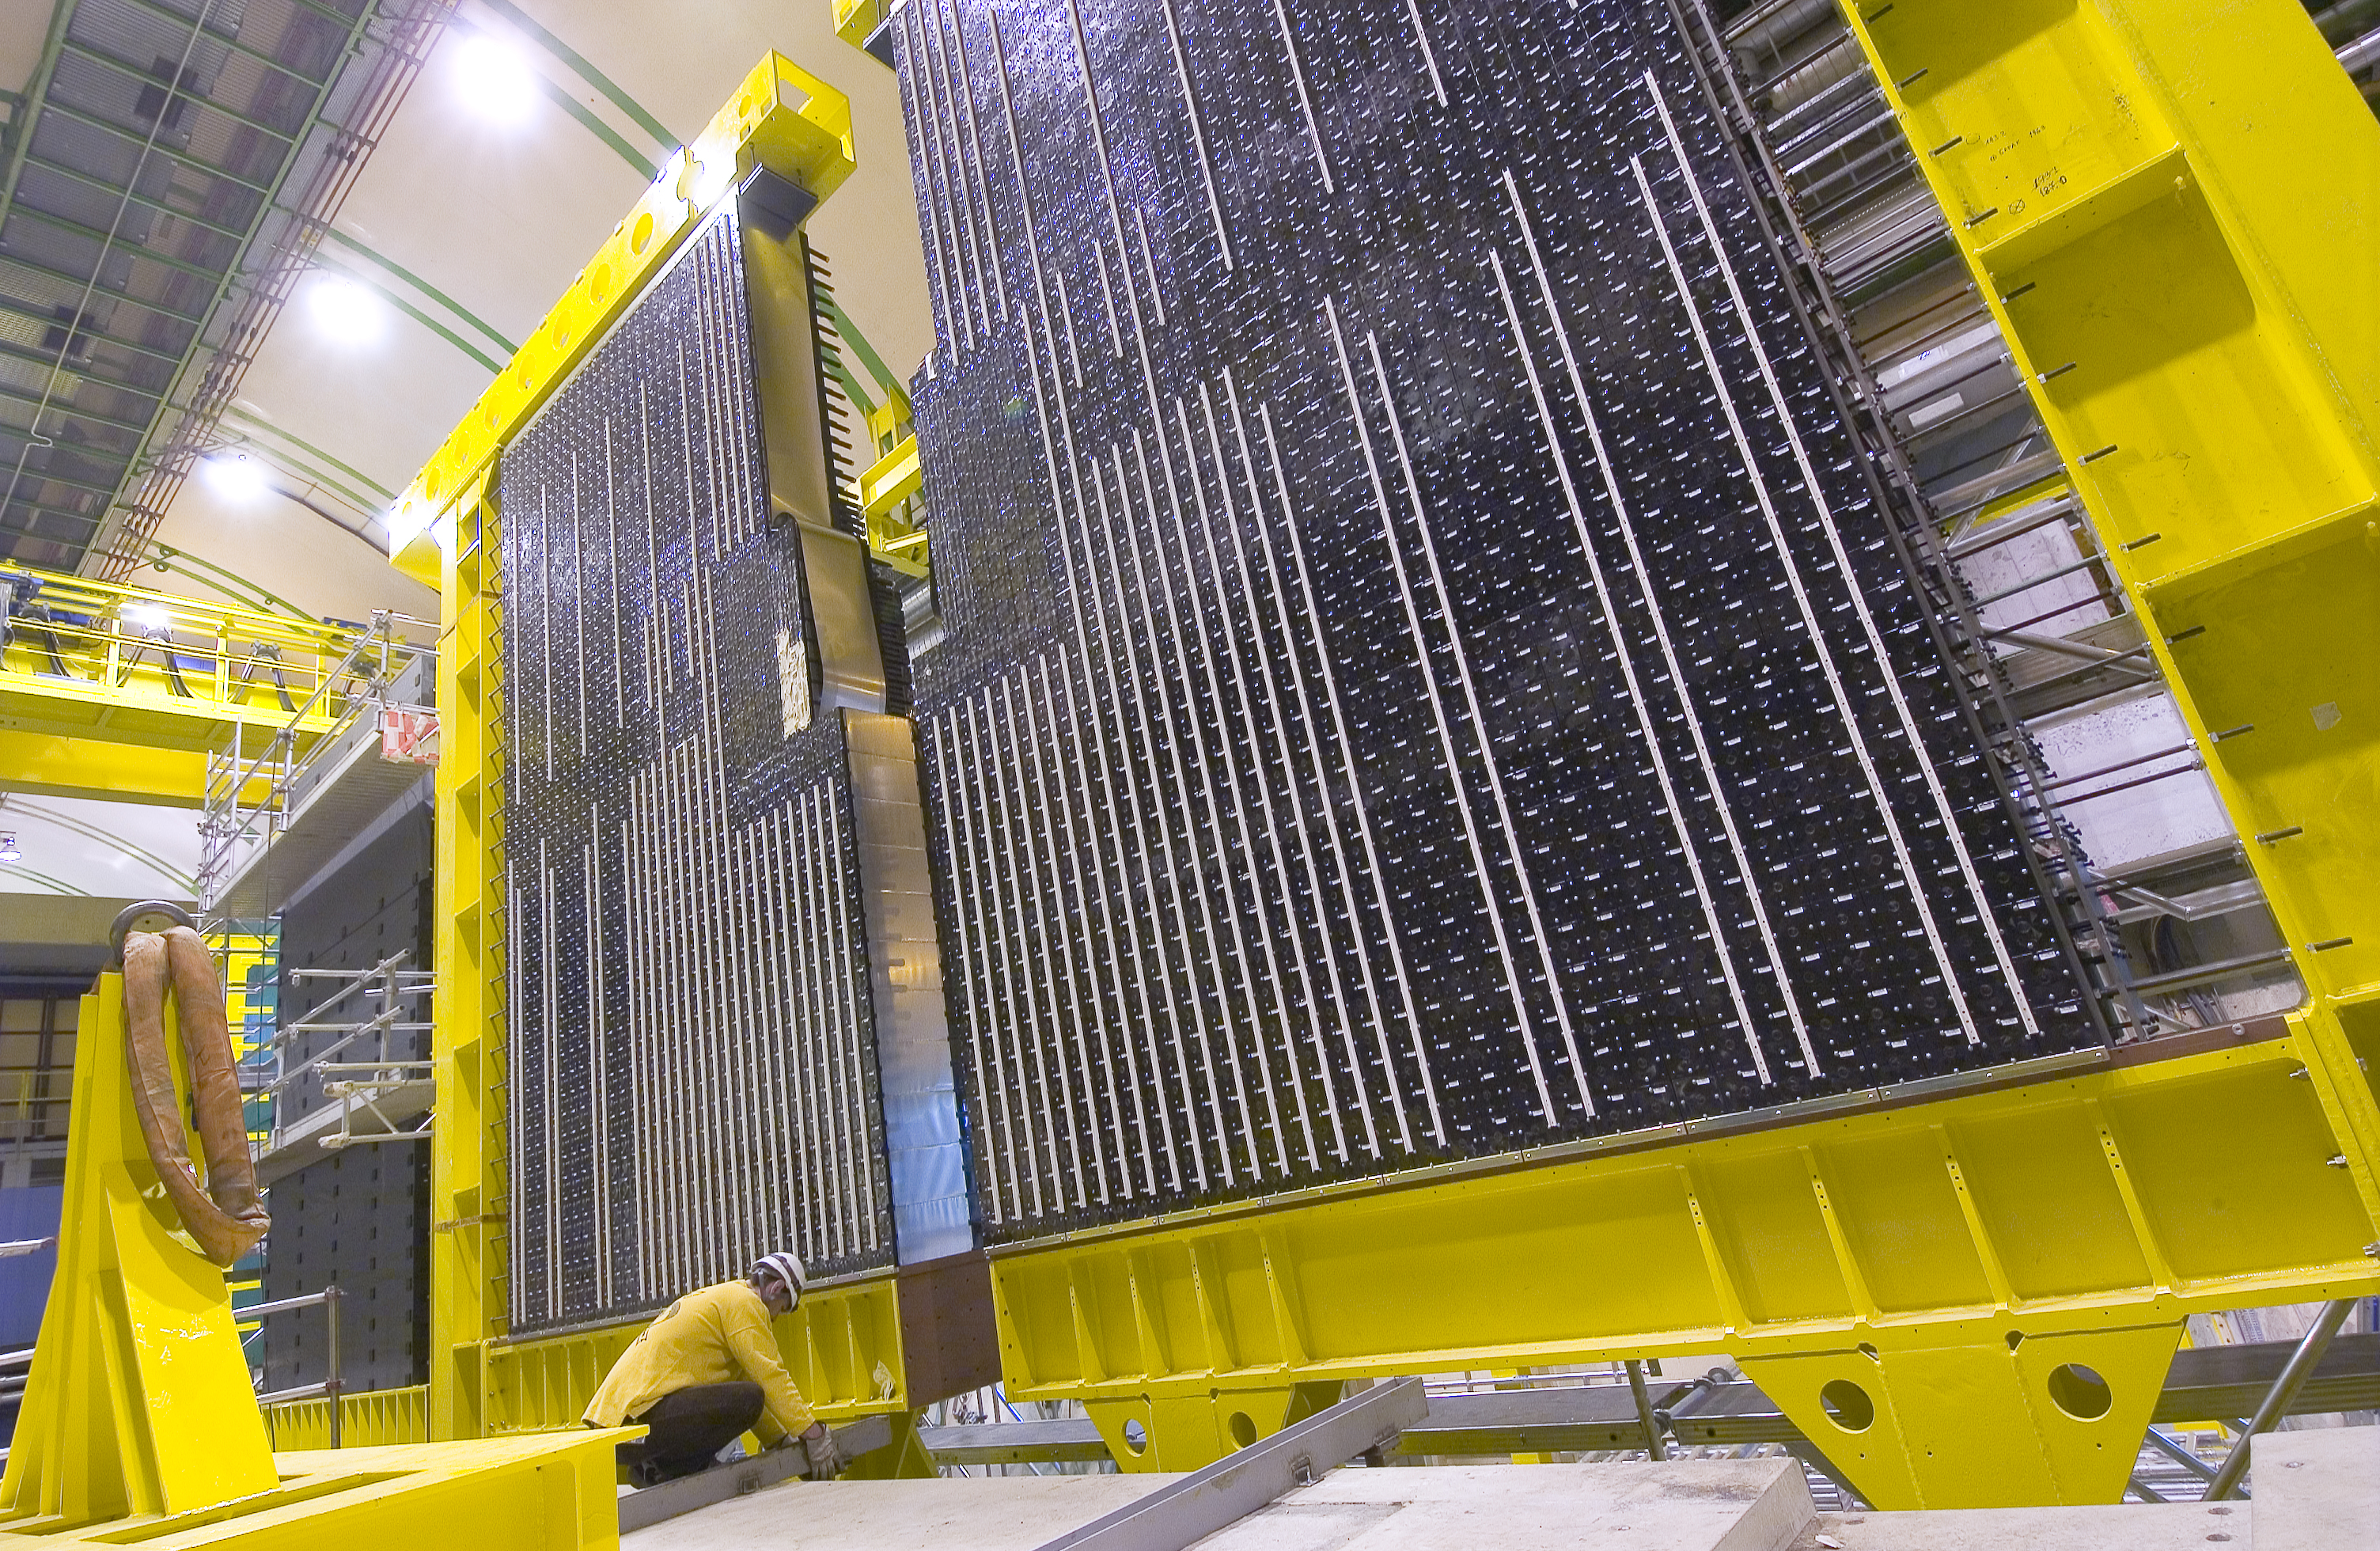
\includegraphics[height=2.5 cm]{Figures Introductory Lecture/LHCb Detector/LHCb_ECAL.JPG}%source:https://cds.cern.ch/record/835712
        \end{figure}
    \end{minipage}
    \vspace{-0.5cm}
    \begin{figure}[h]
    \centering
    \begin{overpic}[width=0.8\textwidth]{Figures Introductory Lecture/LHCb Detector/LHCb_7.png}
               
        \put (55,52) {\colorbox{LHCbDarkBlue!80}{\textcolor{LHCbLightBlue}{\centering \tiny  ECAL}}}
        \put (45.3,52) {\colorbox{lightgray}{\centering \tiny  RICH 2}}
        \put (42,46) {\rotatebox[]{90}{\colorbox{lightgray}{\centering \tiny  T1-T3}}}
        \put (27,52) {\colorbox{lightgray}{\centering \tiny  Magnet}}
        \put (20,40) {\rotatebox[]{90}{\colorbox{lightgray}{\centering \tiny  TT}}}
        \put (13,45) {\colorbox{lightgray}{\centering \tiny  RICH 1}}
        \put (3,35) {\colorbox{lightgray}{\centering \tiny  VELO}}

\put (1,5) {\tiny $z/m \rightarrow$}
\put (17.5,2) {\tiny $2$}
\put (21.4,2) {\tiny $3$}
\put (25.5,2) {\tiny $4$}

\put (39,2) {\tiny $7$}

\put (50,2) {\tiny $10$}
\put (57,2) {\tiny $12$}
 
    \end{overpic}
    \end{figure}
\end{frame}
%%%%%%%%%%%%%%%%%%%%%%%%%%%%%%%%%%%%%%%%%%%%%%%%%%%%%%%%%%%%%%%%%%%%%%%%%%%%%%%%%%%%%%%%%%%%%%
\begin{frame}{Hadronic Calorimeter (HCAL)}
    \begin{minipage}{0.58\textwidth}
    \begin{itemize}
        \item Also stops heavy charged and neutral particles
        \item Measures deposited \textcolor{red}{\textbf{energy}}
    \end{itemize}
    \end{minipage}\hfill
    \begin{minipage}{0.38\textwidth}
        \begin{figure}[h]
        \centering
        \includegraphics[height=2.5 cm]{Figures Introductory Lecture/LHCb Detector/LHCb_HCAL.jpg}%source:https://www.lhc-facts.ch/index.php?page=lhcb dort wird als quelle cern genannt
        \end{figure}
    \end{minipage}
    \vspace{-0.5cm}
    \begin{figure}[h]
    \centering
    \begin{overpic}[width=0.8\textwidth]{Figures Introductory Lecture/LHCb Detector/LHCb_8.png}
        \put (63.5,52) {\colorbox{LHCbDarkBlue!80}{\textcolor{LHCbLightBlue}{\centering \tiny  HCAL}}}
        \put (55,52) {\colorbox{lightgray}{\centering \tiny  ECAL}}
        \put (45.3,52) {\colorbox{lightgray}{\centering \tiny  RICH 2}}
        \put (42,46) {\rotatebox[]{90}{\colorbox{lightgray}{\centering \tiny  T1-T3}}}
        \put (27,52) {\colorbox{lightgray}{\centering \tiny  Magnet}}
        \put (20,40) {\rotatebox[]{90}{\colorbox{lightgray}{\centering \tiny  TT}}}
        \put (13,45) {\colorbox{lightgray}{\centering \tiny  RICH 1}}
        \put (3,35) {\colorbox{lightgray}{\centering \tiny  VELO}}

\put (1,5) {\tiny $z/m \rightarrow$}
\put (17.5,2) {\tiny $2$}
\put (21.4,2) {\tiny $3$}
\put (25.5,2) {\tiny $4$}

\put (39,2) {\tiny $7$}

\put (50,2) {\tiny $10$}
\put (57,2) {\tiny $12$}
\put (65,2) {\tiny $14$}

    \end{overpic}
    \end{figure}
\end{frame}
%%%%%%%%%%%%%%%%%%%%%%%%%%%%%%%%%%%%%%%%%%%%%%%%%%%%%%%%%%%%%%%%%%%%%%%%%%%%%%%%%%%%%%%%%%%%%%
\begin{frame}{Muon Chambers}
    \begin{minipage}{0.58\textwidth}
    \begin{itemize}
        \item Measures \textcolor{red}{\textbf{position}} of muons
    \end{itemize}
    \end{minipage}\hfill
    \begin{minipage}{0.38\textwidth}
        \begin{figure}[h]
        \centering
        \includegraphics[height=2.5 cm]{Figures Introductory Lecture/LHCb Detector/LHCb_Muon.jpg}%source:https://www.lhc-facts.ch/index.php?page=lhcb dort wird als quelle cern genannt
        \end{figure}
    \end{minipage}
    \vspace{-0.5cm}
    \begin{figure}[h]
    \centering
    \begin{overpic}[width=0.8\textwidth]{Figures Introductory Lecture/LHCb Detector/LHCb_9.png}
        \put (85,50) {\colorbox{LHCbDarkBlue!80}{\textcolor{LHCbLightBlue}{\parbox{1.25cm}{\centering \tiny  Muon chambers}}}}
        \put (63.5,52) {\colorbox{lightgray}{\centering \tiny  HCAL}}
        \put (55,52) {\colorbox{lightgray}{\centering \tiny  ECAL}}
        \put (45.3,52) {\colorbox{lightgray}{\centering \tiny  RICH 2}}
        \put (42,46) {\rotatebox[]{90}{\colorbox{lightgray}{\centering \tiny  T1-T3}}}
        \put (27,52) {\colorbox{lightgray}{\centering \tiny  Magnet}}
        \put (20,40) {\rotatebox[]{90}{\colorbox{lightgray}{\centering \tiny  TT}}}
        \put (13,45) {\colorbox{lightgray}{\centering \tiny  RICH 1}}
        \put (7,52) {\colorbox{lightgray}{\centering \tiny  VELO}}

\put (1,5) {\tiny $x/m \rightarrow$}
\put (17.5,2) {\tiny $2$}
\put (21.4,2) {\tiny $3$}
\put (25.5,2) {\tiny $4$}

\put (39,2) {\tiny $7$}

\put (50,2) {\tiny $10$}
\put (57,2) {\tiny $12$}
\put (65,2) {\tiny $14$}
\put (73.5,2) {\tiny $16$}
\put (86,2) {\tiny $20$}
    \end{overpic}
    \end{figure}
\end{frame}
%%%%%%%%%%%%%%%%%%%%%%%%%%%%%%%%%%%%%%%%%%%%%%%%%%%%%%%%%%%%%%%%%%%%%%%%%%%%%%%%%%%%%%%%%%%%%%
\subsection{}
\begin{frame}{Measuring Range of LHCb}
    \begin{figure}[h]
    \centering
    \begin{overpic}[width=\textwidth]{Figures Introductory Lecture/LHCb Detector/LHCb_10.png}
        \put (85,50) {\colorbox{lightgray}{\parbox{1.25cm}{\centering \tiny  Muon chambers}}}
        \put (63.5,52) {\colorbox{lightgray}{\centering \tiny  HCAL}}
        \put (55,52) {\colorbox{lightgray}{\centering \tiny  ECAL}}
        \put (45.3,52) {\colorbox{lightgray}{\centering \tiny  RICH 2}}
        \put (42,46) {\rotatebox[]{90}{\colorbox{lightgray}{\centering \tiny  T1-T3}}}
        \put (27,52) {\colorbox{lightgray}{\centering \tiny  Magnet}}
        \put (20,40) {\rotatebox[]{90}{\colorbox{lightgray}{\centering \tiny  TT}}}
        \put (13,45) {\colorbox{lightgray}{\centering \tiny  RICH 1}}
        \put (3,35) {\colorbox{lightgray}{\centering \tiny  VELO}}

\put (1,5) {\tiny $z/m \rightarrow$}
\put (5,56) {\tiny $y/m$}
\put (17.5,2) {\tiny $2$}
\put (21.4,2) {\tiny $3$}
\put (25.5,2) {\tiny $4$}

\put (39,2) {\tiny $7$}

\put (50,2) {\tiny $10$}
\put (57,2) {\tiny $12$}
\put (65,2) {\tiny $14$}
\put (73.5,2) {\tiny $16$}
\put (86,2) {\tiny $20$} 

\put (7,50.5) {\tiny $+5$} 
\put (6,30.5) {\tiny $0$} 
\put (7,9.5) {\tiny $-5$} 


    \end{overpic}
    \end{figure}
\end{frame}
\subsection{Picture: CERN}
\begin{frame}
    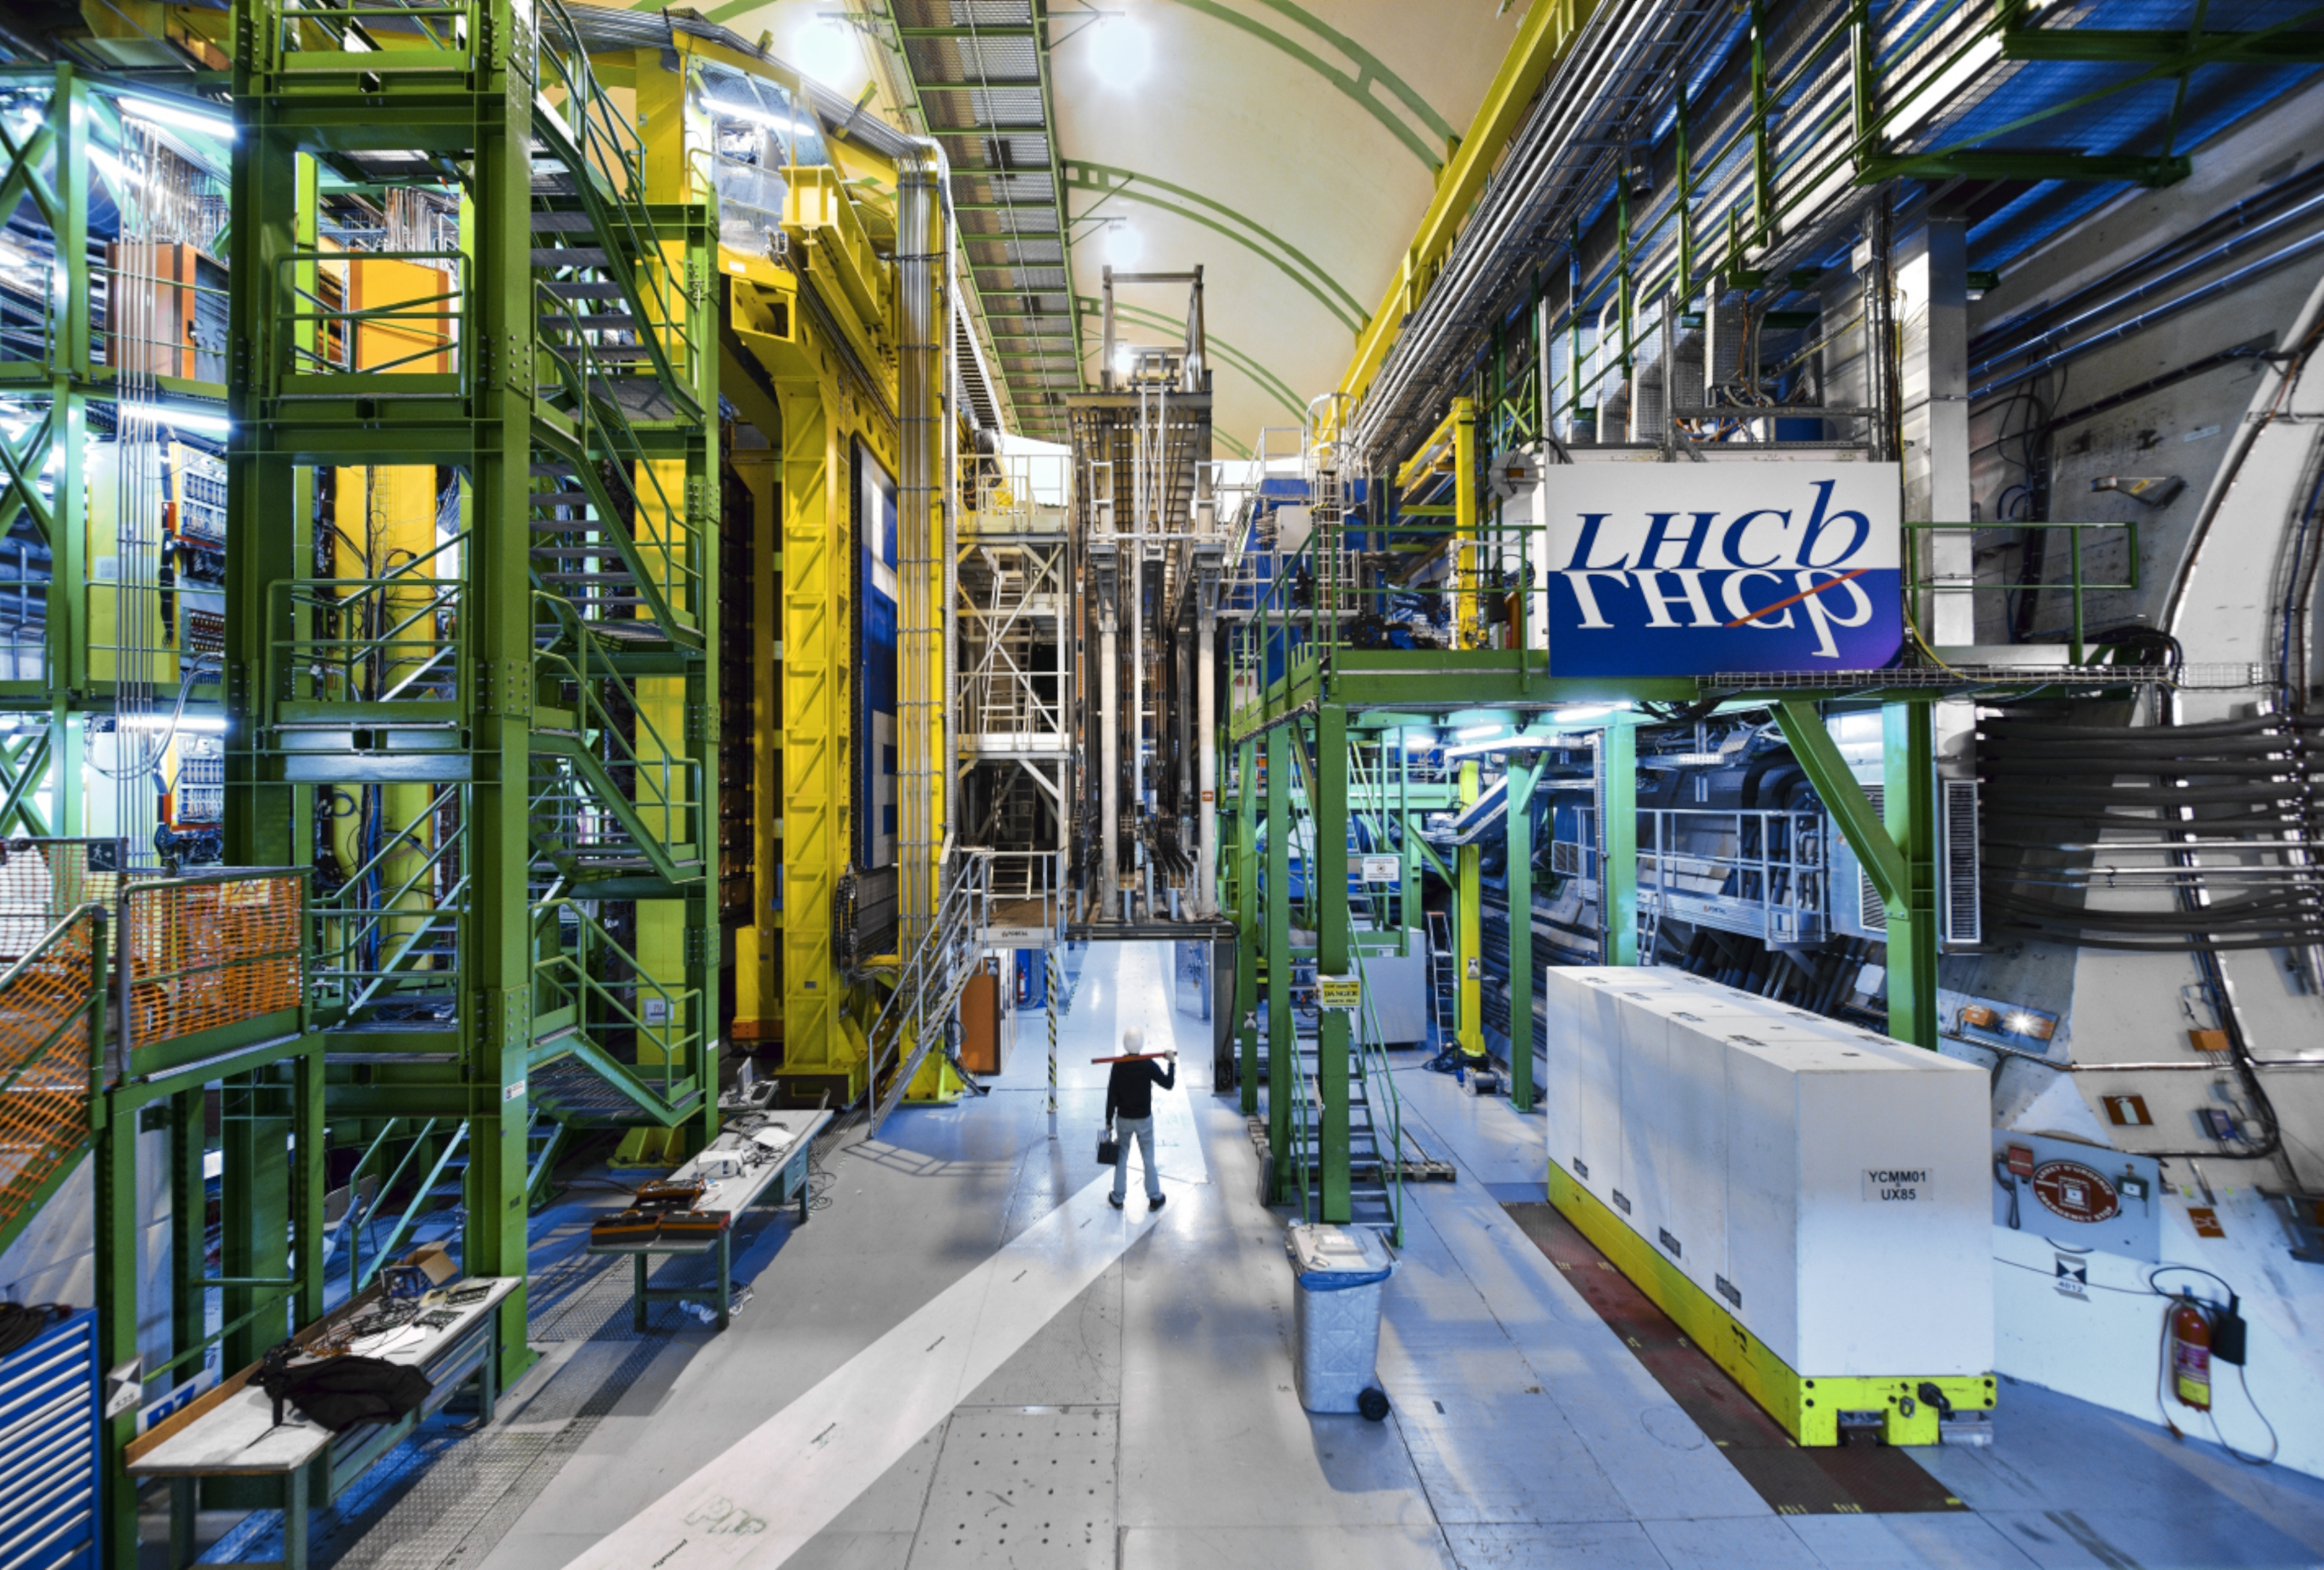
\includegraphics[width=\textwidth]{Figures Introductory Lecture/LHCb Detector/LHCb_image.jpg}
\end{frame}
\begin{frame}
    \begin{overpic}[width=\textwidth]{Figures Introductory Lecture/LHCb Detector/LHCb_image+scheme.jpg.png}
            \put(78,50){\colorbox{lightgray}{\tiny  VELO}}
            \put(73.5,50){\colorbox{lightgray}{\rotatebox[]{90}{\tiny RICH 1}}}
            \put(70.5,50){\colorbox{lightgray}{\rotatebox[]{90}{\tiny TT}}}
            \put(57,60){\colorbox{lightgray}{\tiny Magnet}}
            \put(49,50){\colorbox{lightgray}{\rotatebox[]{90}{\tiny T1-T3}}}
            \put(41,60){\colorbox{lightgray}{\tiny RICH 2}}
            \put(32,60){\colorbox{lightgray}{\tiny ECAL}}
            \put(25,60){\colorbox{lightgray}{\tiny HCAL}}
            \put(11,60){\colorbox{lightgray}{\parbox{1.25cm}{\tiny Muon chambers}}}
                    
    \end{overpic}
\end{frame}
\subsection{}
% \begin{frame}{Was macht wo ein Signal?}
% \begin{figure}[h]
%     \centering
%     \includegraphics[width=\textwidth]{Figures Introductory Lecture/LHCb Detector/Energy Depostition LHCb.png}
%     %\c%aption{%Caption}
%     \label{fig:energy_deposition}
% \end{figure}
% \end{frame}

\begin{frame}{What does a Signal do Where?}
\vspace{-1cm}
\begin{center}
        \begin{tikzpicture}
%Boxen
        \draw[fill=VELO!80, line width=0.01] (0,0)--(0.5,0)--(0.5,5)  to node [black, above]{\rotatebox{90}{\scriptsize VELO}} (0,5) -- (0,0) ;
        \draw[fill=RICH, line width=0.01] (0.7,0)--(1.7,0)--(1.7,5) to node [black, above]{\rotatebox{90}{\scriptsize RICH 1}} (0.7,5)--(0.7,0);
           \draw[fill=gray,line width=0] (1.9,0)--(2.4,0)--(2.4,5) to node [black, above]{\rotatebox{90}{\scriptsize TT}} (1.9,5)-- (1.9,0);
        \draw[fill=Magnet,line width=0] (2.6,0)--(4.3,0)--(4.3,5) to node [black, above]{\rotatebox{90}{\scriptsize Magnet}} (2.6,5)-- (2.6,0);
        \draw[fill=gray,line width=0] (4.5,0)--(5,0)--(5,5)to node [black, above]{\rotatebox{90}{\scriptsize T1-T3}}(4.5,5)-- (4.5,0);
        \draw[fill=RICH,line width=0] (5.2,0)--(6.2,0)--(6.2,5)to node [black, above]{\rotatebox{90}{\scriptsize RICH 2}}(5.2,5)-- (5.2,0);
        \draw[fill=ECAL,line width=0] (6.4,0)--(7.4,0)--(7.4,5)to node [black, above]{\rotatebox{90}{\scriptsize ECAL}}(6.4,5)-- (6.4,0);
        \draw[fill=HCAL,line width=0] (7.6,0)--(8.6,0)--(8.6,5)to node [black, above]{\rotatebox{90}{\parbox{2cm}{\scriptsize HCAL}}}(7.6,5)-- (7.6,0);
                \draw[fill=Muon,line width=0] (8.8,0)--(9.8,0)--(9.8,5)to node [black, above]{\rotatebox{90}{\parbox{1.5cm}{\scriptsize Muon chambers}}}(8.8,5)-- (8.8,0);

%Elektron
        \draw[--, black, line width=0.5mm](-0.5,4) to node[black,left=5pt]{$e^-$} (0,4) to (0.5,4)  (1.9,4) to (2.4,4) (4.5,4.24) to (5,4.32){};
        \draw[--, black, dotted, line width=0.5mm] (0.5,4) to (1.9,4) (2.4,4) to (2.6,4) to [out=0,in=200,bend right=5] (4.3, 4.2) to (4.5,4.24) (5,4.32) to (6.9,4.62);
        \draw[--, red,  line width=2mm,cap=round]  (6.6,4.57) to  (7.2,4.67);

%Antimyon
        \draw[--, black, line width=0.5mm](-0.5,3.5) to node[black,left=5pt]{$\mu^+$} (0,3.5) to (0.5,3.5)  (1.9,3.5) to (2.4,3.5) (4.5,3.26) to (5,3.18)  (6.4,2.9) to (7.4,2.7)(7.6,2.66) to (8.6,2.46) (8.8,2.42) to (9.8,2.22){};
        \draw[--, black, dotted, line width=0.5mm] (0.5,3.5) to (1.9,3.5) (2.4,3.5) to (2.6,3.5) to [out=0,in=200,bend left=5] (4.3, 3.3) to (4.5,3.26) (5,3.18) to (5.2,3.14) to (6.2,2.94) (6.2,2.94) to (6.4,2.9)(7.4,2.7) to (7.6,2.66)(8.6,2.46) to (8.8,2.42);
        \draw[-{Latex[length=3mm]},black,dotted, line width=0.5mm] (9.8,2.22) to (10.3,2.12){};

%Proton
        \draw[--, black, line width=0.5mm](-0.5,3) to node[black,left=10pt]{$p$} (0,3) to (0.5,3)  (1.9,3) to (2.4,3) (4.5,2.76) to (5,2.68)  (6.4,2.4) to (7.4,2.2)(7.6,2.16) (7.6,2.16) to (8.1,2.06){};
        \draw[--, black, dotted, line width=0.5mm] (0.5,3) to (1.9,3) (2.4,3) to (2.6,3) to [out=0,in=200,bend left=5] (4.3, 2.8) to (4.5,2.76) (5,2.68) to (5.2,2.64) to (6.2,2.44) (6.2,2.44) to (6.4,2.4)(7.4,2.2) to (7.6,2.16);
        \draw[--, red,  line width=2mm,cap=round]  (6.8,2.32) to  (7,2.28) (7.8,2.12) -- (8.4,1.98);



%Neutron
        \draw[--, black, dotted, line width=0.5mm](-0.5,1.75) to node[black,left=10pt]{$n$} (0,1.75)  to  (7.6,1.75) {};
        \draw[--, black, line width=0.5mm] (7.6,1.75) to (8.1,1.75) ;
         \draw[--, red,  line width=2mm,cap=round]  (6.8,1.75) to  (7,1.75) (7.8,1.75) -- (8.4,1.75);

%Photon
         \draw[--, black, dotted, line width=0.5mm](-0.5,1.25)  to node[black,left=10pt]{$\gamma$} (0,1.25) to (7.1,1.25) {};
         \draw[--, red,  line width=2mm,cap=round]  (6.6,1.25) to  (7.2,1.25){}; 


%Neutrino
        \draw[-{Latex[length=3mm]}, black,dotted, line width=0.5mm](-0.5,0.75) to node[black,left=10pt]{$\nu$} (0,0.75)  to (10.3,0.75) {};

%Legende
\draw[--, black, dotted, line width=0.5mm](0.5,-0.5) to  node[below, ] {\parbox{2.8cm}{\scriptsize No particle track}} (2.5,-0.5) ;\draw[--, black, line width=0.5mm] (3.5,-0.5) to  node[below, ] {\parbox{2cm}{\scriptsize Particle track\\\ \tiny (due to material alternating effect) }} (5.5,-0.5) ;\draw[--, red,  line width=2mm] (6.5,-0.5) to node[below, black ] {\parbox{2.8cm}{\centering\scriptsize Energy \\ deposition\\ \tiny (particle shower)} } (8.5,-0.5) ;

    \end{tikzpicture}
    \end{center}
\end{frame}
%%%%%%%%%%%%%%%%%%%%%%%%%%%%%%%%%%%%%%%%%%%%%%%%%%%%%%%%%%%%%%%%%%%%%%%%%%%%%%%%%%%%%%%%%%%%%%
\begin{frame}{What does a Measured Event Look Like?}
\begin{figure}[h]
    \centering
    \includegraphics[width=\textwidth]{Figures Introductory Lecture/LHCb Detector/LHCb_Eventdisplay.png}
    %\c%aption{%Caption}
    \label{fig:energy_deposition}
\end{figure}
\end{frame}

%%%%%%%%%%%%%%%%%%%%%%%%%%%%%%%%%%%%%%%%%%%%%%%%%%%%%%%%%%%%%%%%%%%%%%%%%%%%%%%%%%%%%%%%%%%%%%
\newcommand\Bigbullet{\raisebox{-1.1mm}{\scalebox{2.5}{$\bullet$}}}
\newcommand\BigbulletG{\raisebox{-3mm}{\scalebox{5}{$\bullet$}}}

\begin{frame}
Additional slides \Bigbullet


\end{frame}

\begin{frame}{Quark Masses}

    \begin{overpic}[width=1.05\textwidth]{Figures Introductory Lecture/Standard Model/SM_vis_1.png}%
        \put (3.3,15) {\small 2.2\,MeV/$c^2$}
    \end{overpic}
    
\end{frame}

\begin{frame}{Quark Masses}

   \begin{overpic}[width=1.05\textwidth]{Figures Introductory Lecture/Standard Model/SM_vis_2.png}%
        \put (3.6,15) {\centering\footnotesize 2.2\,MeV/$c^2$}
          \put (6,20) {\centering\small 1\,kg}


    \end{overpic}
    
\end{frame}

\begin{frame}{Quark Masses}

   \begin{overpic}[width=1.05\textwidth]{Figures Introductory Lecture/Standard Model/SM_vis_3.png}%
                \put (3.6,15) {\centering\footnotesize 2.2\,MeV/$c^2$}
          \put (6,20) {\centering\small 1\,kg}

          \put (18.6,15) {\centering\footnotesize 4.7\,MeV/$c^2$}
          \put (20,20) {\centering\small $\approx$ 2\,kg}



        

    \end{overpic}
    
\end{frame}
\subsection{Picture: schaette.de}
\begin{frame}{Quark Masses}

   \begin{overpic}[width=1.05\textwidth]{Figures Introductory Lecture/Standard Model/SM_vis_4.png}%
                \put (3.6,15) {\centering\footnotesize 2.2\,MeV/$c^2$}
          \put (6,20) {\centering\small 1\,kg}

          \put (18.6,15) {\centering\footnotesize 4.7\,MeV/$c^2$}
          \put (20,20) {\centering\small $\approx$ 2\,kg}

          \put (32.6,15) {\centering\footnotesize 96\,MeV/$c^2$}
          \put (35,20) {\centering\small $\approx$ 45\,kg}

        

    \end{overpic}
    
\end{frame}
\subsection{Picture: schaette.de $|$ meinhaushalt.at}
\begin{frame}{Quark Masses}

    \begin{overpic}[width=1.05\textwidth]{Figures Introductory Lecture/Standard Model/sm_vis_5.png}%
            \put (3.6,15) {\centering\footnotesize 2.2\,MeV/$c^2$}
          \put (6,20) {\centering\small 1\,kg}

          \put (18.6,15) {\centering\footnotesize 4.7\,MeV/$c^2$}
          \put (20,20) {\centering\small $\approx$ 2\,kg}

          \put (32.6,15) {\centering\footnotesize 96\,MeV/$c^2$}
          \put (35,20) {\centering\small $\approx$ 45\,kg}

        
         \put (48,15) {\centering\footnotesize 1.3\,GeV/$c^2$}
        \put (50,20) {\centering\small $\approx$ 0.6\,t}

   
    \end{overpic}
    
\end{frame}
\subsection{Picture: schaette.de $|$ meinhaushalt.at $|$ M 93 (2021)}
\begin{frame}{Quark Masses}

   \begin{overpic}[width=1.05\textwidth]{Figures Introductory Lecture/Standard Model/SM_vis_6.png}%
        \put (3.6,15) {\centering\footnotesize 2.2\,MeV/$c^2$}
          \put (6,20) {\centering\small 1\,kg}

          \put (18.6,15) {\centering\footnotesize 4.7\,MeV/$c^2$}
          \put (20,20) {\centering\small $\approx$ 2\,kg}

          \put (32.6,15) {\centering\footnotesize 96\,MeV/$c^2$}
          \put (35,20) {\centering\small $\approx$ 45\,kg}

        
         \put (48,15) {\centering\footnotesize 1.3\,GeV/$c^2$}
        \put (50,20) {\centering\small $\approx$ 0.6\,t}

         \put (63,15) {\centering\footnotesize 4.2\,GeV/$c^2$}
          \put (64,20) {\centering\small $\approx$ 1.9\,t}
        
 
    \end{overpic}
    
\end{frame}
\subsection{Picture: schaette.de $|$  meinhaushalt.at $|$ M 93 (2021) $|$ Airbus}
\begin{frame}{Quark Masses}

   \begin{overpic}[width=1.05\textwidth]{Figures Introductory Lecture/Standard Model/SM_vis_7.png}%
        \put (3.6,15) {\centering\footnotesize 2.2\,MeV/$c^2$}
          \put (6,20) {\centering\small 1\,kg}

          \put (18.6,15) {\centering\footnotesize 4.7\,MeV/$c^2$}
          \put (20,20) {\centering\small $\approx$ 2\,kg}

          \put (32.6,15) {\centering\footnotesize 96\,MeV/$c^2$}
          \put (35,20) {\centering\small $\approx$ 45\,kg}

        
         \put (48,15) {\centering\footnotesize 1.3\,GeV/$c^2$}
        \put (50,20) {\centering\small $\approx$ 0.6\,t}

         \put (63,15) {\centering\footnotesize 4.2\,GeV/$c^2$}
          \put (64,20) {\centering\small $\approx$ 1.9\,t}
        
        \put (77,15) {\centering\footnotesize 173\,GeV/$c^2$}
        \put (78,20) {\centering\small $\approx$ 79\,t}

    \end{overpic}
    
\end{frame}
\subsection{}
\begin{frame}
\begin{minipage} {0.3\textwidth}
\includegraphics[width=\textwidth]{Figures Introductory Lecture/Standard Model/Hadron_coloured.png}
\end{minipage}
\begin{minipage} {0.65\textwidth}
Simple consideration:\\  $m\big( \textcolor{lightgray}{ \BigbulletG}\big)\overset{?}{=}m(\textcolor{red}{\Bigbullet})+m(\textcolor{blue}{\Bigbullet})+m(\textcolor{green}{\Bigbullet})$
\end{minipage}
e.g. proton ($uud$):\\
\begin{align*} 
m(u)&=2.2  \,\textmd{ MeV}/c^2\\m(d)&= 4.7 \, \textmd{ MeV}/c^2 \\ \rightarrow m(\textmd{Proton})&=9.1  \,\textmd{ MeV}/c^2
\end{align*} 
In fact, one finds:
\begin{align*} 
m(\textmd{Proton})=938  \,\textmd{ MeV}/c^2
\end{align*} 
\end{frame}
\begin{frame}\addtocounter{framenumber}{-1}
\begin{minipage} {0.3\textwidth}
\includegraphics[width=\textwidth]{Figures Introductory Lecture/Standard Model/Hadron_seequarks_coloured.png}
\end{minipage}
\begin{minipage} {0.65\textwidth}
Simple consideration:\\  $m\big( \textcolor{lightgray}{ \BigbulletG}\big)\neq m(\textcolor{red}{\Bigbullet})+m(\textcolor{blue}{\Bigbullet})+m(\textcolor{green}{\Bigbullet})$
\end{minipage}
e.g. proton ($uud$):\\
\begin{align*} 
m(u)&=2.2  \,\textmd{ MeV}/c^2\\m(d)&= 4.7 \, \textmd{ MeV}/c^2 \\ \rightarrow m(\textmd{Proton})&=9.1  \,\textmd{ MeV}/c^2
\end{align*} 
In fact, one finds:
\begin{align*} 
m(\textmd{Proton})=938  \,\textmd{ MeV}/c^2
\end{align*} 
\end{frame}
\begin{frame}{References}\scriptsize
\begin{itemize}
\item[-] Maximilien Brice/CERN (2018) \url{https://cds.cern.ch/images/CERN-PHOTO-201801-025-18/} 
\item[-] Maximilien Brice/CERN (2008). \url{cds.cern.ch/record/1295244}
\item[-] Paula Collins/CERN (2007)  \url{cds.cern.ch/record/1017398}
\item[-] Christoph Frei/CERN (2021)  \url{cds.cern.ch/record/2807064}
\item[-] Angela Buechler/CERN (2009)  \url{twiki.cern.ch/twiki/bin/view/LHCb/ConferenceSummaryIEEFlorida2009}
\item[-] Peter Ginter/CERN (2008) \url{cds.cern.ch/record/1124307}
\item[-] Maximilien Brice, Julien Ordan/CERN (2009)  \url{facebook.com/LHCbExperiment/photos/a.238680152959433/1123439814483458/?type=3}
\item[-] Maximilien Brice, Julien Ordan/CERN (2009)  \url{https://cds.cern.ch/record/2302374}
\item[-] CERN (2015). \url{https://lhcb.web.cern.ch/lhcb_page/collaboration/LHCb20/ }
\item[-] Maximilien Brice/CERN (2005)  \url{cds.cern.ch/record/835712}
\item[-] schaette.de. \url{schaette.de/ratgeber/tiergesundheit/rinder/rinder-was-koennen-wir-fuer-abwehrstarke-kaelber-tun}
\item[-] meinhaushalt.at (2009). \url{meinhaushalt.at/4182-zunge-schalen-kochen/#}
\item[-] M 93 (2021) BMW X3 xDrive20d xLine (G01) – h 02042021.jpg
\item[-] Airbus. \url{aircraft.airbus.com/en/aircraft/a320/a321xlr#images}
\end{itemize}
\end{frame}
\end{document}